\documentclass[tikz,border=10pt]{standalone}
\usepackage{tikz}
\usetikzlibrary{matrix}

\tikzset{
  cell/.style={draw=black!70, line width=1.0pt, minimum width=4.8cm, minimum height=1.2cm, align=center, text width=4.4cm, fill=none},
  head/.style={cell, draw=blue!70!black, line width=1.2pt},
  left/.style={cell, draw=green!50!black, line width=1.2pt}
}

\begin{document}
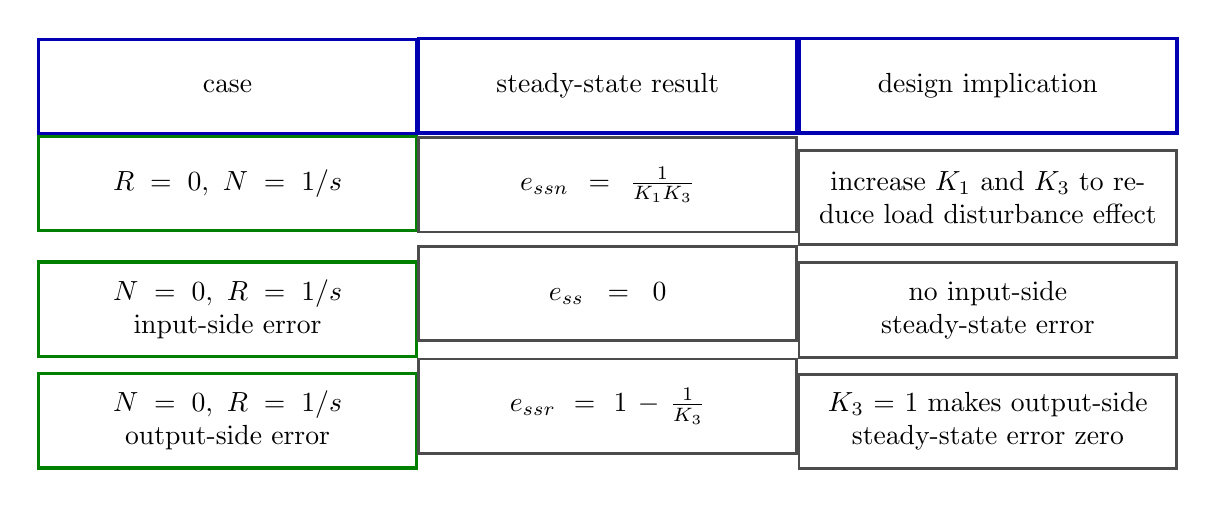
\begin{tikzpicture}
  \matrix[matrix of nodes, nodes in empty cells, row sep=-\pgflinewidth, column sep=-\pgflinewidth] {
    \node[head] {case}; &
    \node[head] {steady-state result}; &
    \node[head] {design implication}; \\
    \node[left] {$R=0,\ N=1/s$}; &
    \node[cell] {$e_{ssn}=\frac{1}{K_1K_3}$}; &
    \node[cell] {increase $K_1$ and $K_3$ to reduce load disturbance effect}; \\
    \node[left] {$N=0,\ R=1/s$\\input-side error}; &
    \node[cell] {$e_{ss}=0$}; &
    \node[cell] {no input-side steady-state error}; \\
    \node[left] {$N=0,\ R=1/s$\\output-side error}; &
    \node[cell] {$e_{ssr}=1-\frac{1}{K_3}$}; &
    \node[cell] {$K_3=1$ makes output-side steady-state error zero}; \\
  };
\end{tikzpicture}
\end{document}
